% !TEX root = ../main.tex
\paragraph{Particle Identification}
% --+ Introduction +------------------------------------------------------------
    The Particle Identification (PID) numbering scheme presented here was introduced by the Particle Data Group (PDG) in 1988 \cite{yost1988}.
    It is intended to aid in interfacing between the various generators, simulators, and analysis packages used in particle physics.
    The system was then revised and adapted in 1998 to allow the systematic inclusion of undiscovered and hypothetical particles \cite{particle1998}.
    The system used in this thesis comes from the most recent version as of the writing of this document, cited from the 2020 Review of Particle Physics by the PDG \cite{particle2020review}.

    The Event Builder (EB) is a service in the reconstruction chain, and performs a series of functions:
    It collects information from the upstream services; correlates information from the sub-detectors into particles; performs a general particle identification scheme; and organises the resulting information into a standardised, persistent data bank structure.
    The service is run twice with identical algorithms, once using hit-based tracks, and later with time-based tracks.
    As mentioned before, the results of the hit-based EB are used to initialise time-based tracking.

% --+ Forming particles +-------------------------------------------------------
    In defining a reconstructed charged particle in CLAS12, the EB assumes that an assignment will be made for each reconstructed track in both the FD and the CD.
    The associated calorimeter, scintillator, and Cherenkov detector responses are then assigned to that particle based on geometric coincidences between the detector responses and the track, with matching criteria corresponding to the resolution of a given detector.
    The geometric matching is based on the DOCA between the track and the response.
    A similar procedure is followed for creating neutral particles, except the seeding is presently with unassociated ECAL for the FD and CND for the CD responses instead of tracks.

% --+ Event start time +--------------------------------------------------------
    A start time is assigned to the entire event and serves as the most precise reference time on which all time-based particle identification relies.
    This is based on the optimal charged particle candidate in the FD with an associated FTOF timing response.
    The EB assigns the start time based on the highest energy electron in the ECAL.
    If there is no electron in the ECAL, it next looks for a positron in the ECAL.
    If there is no lepton, the next track in the priority list is a forward-going positive track (assumed to be a $\pi+$).
    Finally, if there is no forward-going positive track, it looks for a forward-going negative
    track (assumed to be a $\pi-$).
    When looking for $\pi+$ or $\pi-$ tracks, only the candidate with the highest momentum in each group is considered.

    A parallel event start time is determined from the FT to facilitate physics analyses and triggers where the primary scattered electron is at very forward angles in the FT.
    In this case, all combinations of charged particles in the FT and the FD are considered.
    The particle in the FT is assumed to be an electron, whereas all hadron mass hypotheses are considered for the FD tracks.
    The combination with the best time coincidence is chosen.
    The timing of the resulting FT electron is then used to assign the start time.
    A correction to the start time is then performed using the Radio Frequency (RF) signal from the accelerator, combined with the reconstructed event vertex position.
    This effectively aligns the event start time to the best measure of the beam-bunch arrival time at the target.
    The uncorrected, measured vertex time of a particle, $t_v$, can be written as
    \begin{equation*}
        t_v = t - \frac{P_L}{\beta c},
    \end{equation*}
    where $t$ is the measured time response (e.g. in a scintillator), $P_L$ is the path length between the primary interaction vertex and that response, and $\beta c$ is the speed of the particle.

    Then, we find the time difference $\Delta t_{RF}$ between this $t_v$ and the closest beam bunch using
    \begin{equation*}
        \Delta t_{RF} = t_v + \frac{z_0 - z_v}{c} - t_{RF} - \frac{N}{2f_{RF}},
    \end{equation*}
    $z_v$ is the event vertex position's $z$-coordinate, while $z_0$ is the target center, which is used as a position calibration reference, and $c$ is the speed of light in vacuum.
    $t_{RF}$ and $f_{RF}$ are the measured and calibrated RF time and frequency of the accelerator.
    They can be either $2.004 \text{ns}$ and $249.5 \text{MHz}$, or $4.008 \text{ns}$ and $499 \text{MHz}$, respectively.
    When doing reconstruction, they are read from the Run Conditions Database (RCDB).

    This time can then be corrected to the closest beam bunch
    \begin{equation*}
        \Delta t^\prime_{RF} = \text{mod}\left(\Delta t_{RF}, \frac{1}{f_{RF}}\right) - \frac{1}{2f_{RF}},
    \end{equation*}
    which allows us to do RF-correction to $t_v$.
    We now have a final RF- and vertex-corrected start time for the event, defined as
    \begin{equation*}
        t' = t_v - \Delta t^\prime_{RF}.
    \end{equation*}

% --+ Particle identification +-------------------------------------------------
    The next stage is a basic particle identification scheme.
    This is intended to be loose to accommodate a variety of physics analyses, while persisting the necessary information to easily tighten and improve the criteria later.
    For charged particles, first calorimetry and Cherenkov information is used to positively identify $e-/e+$ candidates in the FD.
    If the measured energy deposition is consistent with the expected sampling fraction of the ECAL, and the photoelectron response from the HTCC is consistent with $\beta \sim 1$, the particle is assigned as an $e-$ or $e+$ depending on sign of the curvature of the track from forward tracking with the DCs through the torus magnetic field.

    The remaining charged particles are then assumed to be hadrons and assigned an identity based solely on timing information, where the $p,K,\pi$ candidate giving the smallest time residual is assigned.
    This time residual is computed from the difference between the measured particle flight time and that computed for a given mass hypothesis.

    \begin{wrapfigure}{r}{0.49\textwidth}
        \centering\frame{
        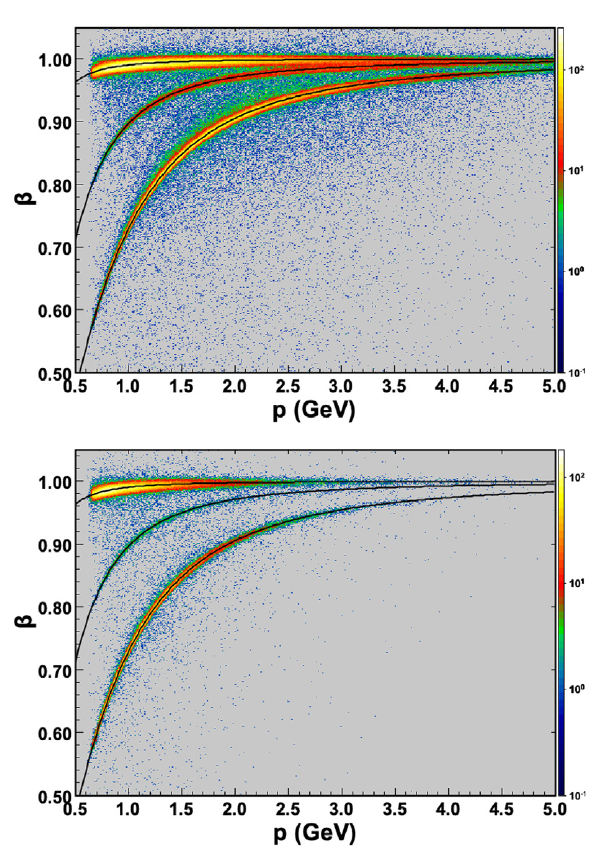
\includegraphics[width=\linewidth]{11experiment/img/23pos_pid.png}}
        \caption[Particle $\beta$ vs. momentum for positively charged tracks.]{Particle $\beta$ vs. momentum from simulation data for positively charged tracks with their start time from an electron in the FD (top plot) or in the FT (bottom plot).}
        \label{fig::pos_pid}
    \end{wrapfigure}

    Figure \ref{fig::pos_pid} shows reconstructed $\beta$ vs. momentum distributions from beam data for forward-going positively charged hadrons using information from the FTOF and DC subsystems, where the electron is reconstructed either in the FD (top) or in the FT (bottom).
    The computed curves for the different mass hypotheses are overlaid.

    Identification of neutral particles assumes only neutrons and photons, differentiated only by timing and topological information.
    For the FD this is based on the ECAL, while for the CD it is based on the CND, and their reconstructed cluster positions are used to compute the particle travel path from the event vertex, assuming a straight-line trajectory.
    If the resulting measured $\beta$ is close to $1$, the particle is assigned as a photon, otherwise it is assigned as a neutron.
    For photons in the FD, the momentum is determined from its deposited energy and ECAL sampling fraction \cite{asryan2020}.
    For neutrons, the momentum is assigned based on the measured $\beta$, assuming the neutron mass.
    Figure \ref{fig::n_gamma} shows an example of $\beta$ reconstructed for neutrals in the FD showing separation of photons and neutrons.

    \begin{wrapfigure}{r}{0.50\textwidth}
        \centering\frame{
        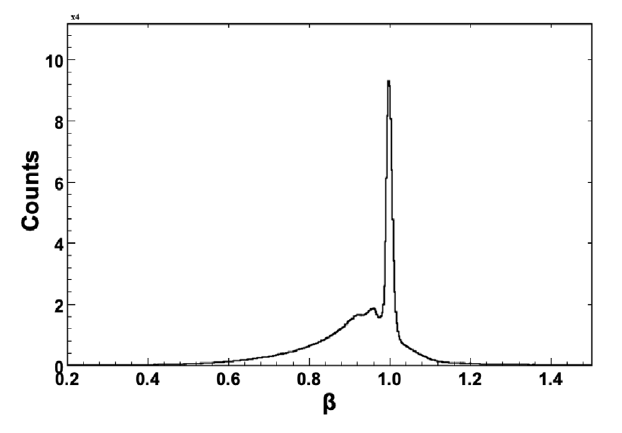
\includegraphics[width=\linewidth]{11experiment/img/23n_gamma.png}}
        \caption[$\beta$ distribution of neutrals.]{$\beta$ distribution for neutral particles as measured by the ECAL from simulation data, showing a sharp peak at $\beta = 1$ from photons and a broader, slower distribution from neutrons.
        }
        \label{fig::n_gamma}
    \end{wrapfigure}

% --+ Particle identification performance +-------------------------------------
    A particle identification quality factor in the form of a signed-$\chi^2$, or pull, is assigned based on the individual contributing detector subsystem responses and their resolutions.
    For $e-/e+$ identification the resolution-normalised distance from the expected ECAL sampling fraction is used, while for charged hadrons the resolution normalised time-difference is used.
    The resulting information is organised into standardised output bank structures for physics analysis.
    This includes the particle four-vectors, the associated detector responses, and global event information such as beam RF and helicity information.

    The accuracy of the particle identification algorithm that is currently implemented can be estimated from Monte Carlo simulations where the assigned particle identification can be compared to the true one.
    Table \ref{tab::rpid} shows the particle identification matrix for the FD (left) and CD (right).
    The values are based on simulations of electron-hadron or electron-photon pairs with hadron and photon momenta in the range from $1$ to $2.5 \text{GeV}$ and electron momenta in the range from $1$ to $9 \text{GeV}$.
    The diagonal elements correspond to the cases where the particle is correctly identified and the off-diagonal elements to the cases where the particle is misidentified ~\cite{ziegler2020}.
    % Another measure of the particle identification performance for neutrals is given by the reconstruction of $\pi^0$ decays to two photons.

    \begin{table}
        \caption{Particle identification matrix for the FD (left matrix) and CD (right matrix).
        The FD matrix is based on simulated hadrons and photons with momentum between $1$ and $2.5~\text{GeV}$, and electrons up to $9~\text{GeV}$.
        The CD matrix is based on simulated hadrons with momentum between $0.3$ and $1.1~\text{GeV}$.
        The diagonal elements are correctly identified, while the off-diagonal elements are misidentified.
        Detector inefficiencies are included.}

        \begin{tabularx}{\textwidth}{XXXXXXX|XXXXX}
            \hline
                     & \multicolumn{6}{l}{\textit{FD Truth}} & \multicolumn{5}{l}{\textit{CD Truth}}  \\
            \cline{2-12}
                     & $e$      & $\pi$ & $K$  & $p$  & $n$  & $\gamma$ &       & $\pi$    & $K$  & $p$  & $n$  \\
            \hline
            $e$      & 0.98     &       &      &      &      &          &       &          &      &      &      \\
            $\pi$    &          & 0.93  & 0.10 & 0.00 &      &          & $\pi$ & 0.84     & 0.14 & 0.00 &      \\
            $K$      &          & 0.03  & 0.80 & 0.00 &      &          & $K$   & 0.11     & 0.80 & 0.01 &      \\
            $p$      &          & 0.03  & 0.02 & 0.98 &      &          & $p$   & 0.03     & 0.04 & 0.95 &      \\
            $n$      &          &       &      &      & 0.66 & 0.01     & $n$   &          &      &      & 0.11 \\
            $\gamma$ &          &       &      &      & 0.14 & 0.95     &       &          &      &      &      \\
            \hline
        \end{tabularx}
        \label{tab::rpid}
    \end{table}
